%% FEUP THESIS STYLE for LaTeX2e
%% how to use feupteses (portuguese version)
%%
%% FEUP, JCL & JCF, 31 Jul 2012
%%
%% PLEASE send improvements to jlopes at fe.up.pt and to jcf at fe.up.pt
%%

%%========================================
%% Commands: pdflatex tese
%%           bibtex tese
%%           makeindex tese (only if creating an index) 
%%           pdflatex tese
%% Alternative:
%%          latexmk -pdf tese.tex
%%========================================

\documentclass[11pt,a4paper,twoside,openright]{report}

%% For iso-8859-1 (latin1), comment next line and uncomment the second line
\usepackage[utf8]{inputenc}
%\usepackage[latin1]{inputenc}

%% Portuguese version

%% MIEIC options
\usepackage[portugues,mieic]{feupteses}
%\usepackage[portugues,mieic,juri]{feupteses}
%\usepackage[portugues,mieic,final]{feupteses}
%\usepackage[portugues,mieic,final,onpaper]{feupteses}

%% Options: 
%% - portugues: titles, etc in portuguese
%% - onpaper: links are not shown (for paper versions)
%% - backrefs: include back references from bibliography to citation place

%% Uncomment the next lines if side by side graphics used
%\usepackage[lofdepth,lotdepth]{subfig}
%\usepackage{graphicx}
%\usepackage{float}

%% Include color package
\usepackage{color}
\definecolor{cloudwhite}{cmyk}{0,0,0,0.025}

\usepackage{multirow}

%% Include source-code listings package
\usepackage{listings}
\lstset{ %
 language=C,                        % choose the language of the code
 basicstyle=\footnotesize\ttfamily,
 keywordstyle=\bfseries,
 numbers=left,                      % where to put the line-numbers
 numberstyle=\scriptsize\texttt,    % the size of the fonts that are used for the line-numbers
 stepnumber=1,                      % the step between two line-numbers. If it's 1 each line will be numbered
 numbersep=8pt,                     % how far the line-numbers are from the code
 frame=tb,
 float=htb,
 aboveskip=8mm,
 belowskip=4mm,
 backgroundcolor=\color{cloudwhite},
 showspaces=false,                  % show spaces adding particular underscores
 showstringspaces=false,            % underline spaces within strings
 showtabs=false,                    % show tabs within strings adding particular underscores
 tabsize=2,	                    % sets default tabsize to 2 spaces
 captionpos=b,                      % sets the caption-position to bottom
 breaklines=true,                   % sets automatic line breaking
 breakatwhitespace=false,           % sets if automatic breaks should only happen at whitespace
 escapeinside={\%*}{*)},            % if you want to add a comment within your code
 morekeywords={*,var,template,new}  % if you want to add more keywords to the set
}

%% Uncomment next line to set the depth of sectional units listed in the toc
%\setcounter{tocdepth}{3}

%% Uncomment to create an index (at the end of the document)
%\makeindex

%% Path to the figures directory
%% TIP: use folder ``figures'' to keep all your figures
\graphicspath{{figures/}}

%%----------------------------------------
%% TIP: if you want to define more macros, use an external file to keep them
%some macro definitions

% format
\newcommand{\class}[1]{{\normalfont\slshape #1\/}}

% entities
\newcommand{\Feup}{Faculdade de Engenharia da Universidade do Porto}

\newcommand{\scada}{\class{SCADA}}
\newcommand{\scadadms}{\class{SCADA/DMS}}
\newcommand{\web}{\textit{web} }

%%----------------------------------------

%%========================================
%% Start of document
%%========================================
\begin{document}

%%----------------------------------------
%% Information about the work
%%----------------------------------------
\title{Estudo, conceção, desenvolvimento e teste de uma aplicação móvel de pagamento e validação para Transportes Públicos de Passageiros}
\author{André Gonçalves Dias}

%% Uncomment next line for date of submission
%\thesisdate{31 de Julho de 2008}

%% Uncomment next line for copyright text if used
%\copyrightnotice{Nome do Autor, 2008}

\supervisor{Orientador}{João Bernardo de Sena Esteves Falcão e Cunha}

%% Uncomment next line if necessary
\supervisor{Co-orientador}{Marta Maria Campos Ferreira}

%% Uncomment committee stuff in the final version
%\committeetext{Aprovado em provas públicas pelo Júri:}
%\committeemember{Presidente}{Nome do presidente do júri}
%\committeemember{Arguente}{Nome do arguente do júri}
%\committeemember{Vogal}{Nome do vogal do júri}
%\signature

%% Specify cover logo (in folder ``figures'')
\logo{uporto-feup.pdf}

%% Uncomment next line for additional text below the author's name (front page)
%\additionalfronttext{Preparação da Dissertação}

%%----------------------------------------
%% Preliminary materials
%%----------------------------------------

% remove unnecessary \include{} commands
\begin{Prolog}
  \chapter*{Resumo}

O uso de dispositivos móveis faz cada vez mais parte do dia-a-dia dos seres humanos. O telemóvel, o leitor de .mp3, o \textit{tablet}, o GPS, a câmara fotográfica, etc. passaram a ser objetos comuns nos bolsos e carteiras. É precisamente devido às capacidades dos \textit{smartphones}, os telemóveis inteligentes que vieram revolucionar a forma como o telemóvel é visto, deixando este de ser apenas um utensílio para a realização de chamadas e envio de mensagens de texto passando para um sistema completo de agenda, telefone, reprodutor multimédia, câmara fotográfica, navegador GPS, entre muitas outras funcionalidades, que surge a pergunta: Se o telemóvel suporta todas estas funcionalidades, porque não utilizá-lo também para uma das tarefas mais rotineiras de muitas pessoas, os transportes públicos?
\\Apesar de, em Portugal, ser já comum utilizar-se sistemas informatizados e relativamente sofisticados no que toca aos sistemas de bilhética nos transportes públicos, estes estão ainda “presos” a cartões, no Grande Porto o cartão Andante, na Grande Lisboa o cartão Viva, nos comboios o cartão CP. Será a informação armazenada nos cartões demasiado complexa que não possa ser armazenada noutro meio, nomeadamente o telemóvel? A resposta é óbvia, Não! A informação armazenada limita-se ao número de títulos de viagem disponíveis naquele cartão e em caso de um título estar ativo, qual o seu período de validade e a estação de entrada. Toda esta informação pode ser facilmente armazenada no telemóvel, sendo apenas necessário implementar as infraestruturas tecnológicas que deem suporte a este novo modelo.
\\O objetivo deste projeto é precisamente estudar e conceber a melhor maneira de tirar partido dos telemóveis para substituir os cartões no que toca à bilhética nos transportes públicos da Área Metropolitana do Porto. Isto permitirá não só aumentar a comodidade do passageiro, como proporcionar-lhe um acesso ilimitado e independente de local ou hora a todos os serviços necessários na gestão da sua mobilidade. Estes serviços incluem a compra de títulos de viagem e sua posterior validação, a consulta do saldo da carteira virtual e o saldo de viagens, a visualização do histórico de operações, a visualização do estado atual da viagem validada (tempo restante e estação de entrada, número de zonas, etc.), entre outros.
\\Mas não é só o passageiro que fica a ganhar. Os operadores de transportes públicos de passageiros, para além de acrescentarem valor à sua oferta de serviços, reduzem custos de operação e manutenção, recolhem informação estatística e hábitos de utilização dos passageiros, e mostram vontade de estar na vanguarda no que toca à inovação tecnológica. Existem já vários projetos piloto em execução em vários países, testando tecnologias diferentes, em busca da melhor solução. É importante referir que cada rede de transportes públicos é única e com características especiais, pelo que não será nunca possível encontrar uma solução que sirva todos os modelos utilizados, sendo necessário desenhar uma solução adequada às necessidades de cada rede.
\\O sistema de bilhética móvel para a Área Metropolitana do Porto não só foi desenvolvido como também foi testado com utilizadores reais cujo contributo foi importante para identificar problemas e sugestões de melhoria e testar o conceito de compra e validação de bilhetes através do telemóvel.

\chapter*{Abstract}

The use of mobile devices is more and more a daily routine of human beings. Mobile phones, .mp3 players, tablets, GPS, cameras, etc. are now ordinary objects in pockets or bags. It's precisely due to the capacities of smartphones, the smart mobile phones that revolutionized the way mobile phones are seen, no longer being just a tool to make calls and send text messages, and becoming a complete system of diary, phone, multimedia player, camera, GPS navigator, among others, that arises the question: “If smartphones support all these functionalities, why not use it on one daily task for most people, public transportation?”.
\\Although, in Portugal, the use of computerized and relatively sophisticated systems in public transportation ticketing is now a common practice, it is still “stuck” to cards. In Oporto, there is the Andante card, in Lisbon the Viva card and in trains, the CP card. Is the stored information so complex that it couldn’t be stored anywhere else, for instance in a smartphone? The answer is obvious, No! The stored information is only the number of remaining traveling titles in that card, and in case one title is active, the expiration time and departure station. All this information can be easily stored in a smartphone, with only the need to develop the technological infrastructures to support this model.
\\The aim of this project is precisely to study and conceive the best way to take advantage of smartphones to replace cards in the Oporto Metropolitan Area public transportation system. This would not only increase passenger’s commodity but also provide him an unlimited and place and time independent access to all the needed services related to his mobility management. These services include purchasing traveling titles, and validating them, checking the virtual wallet balance and the titles balance, visualizing the operations history, visualizing the status of an active title (remaining time, departure station, number of zones, etc.), among others.
\\But the passenger is not the only one who benefits. The passengers public transportation operators, besides adding value to their services offer, reduce operation and maintenance costs, and gather statistical information and use habits from their customers. Moreover, they show the will to be in the edge of technological innovation. There are already some pilot projects running in different countries, searching for the best solution. It is important to have in mind that each public transportation network is unique and with special characteristics, so it will never be possible to find a general solution that fits every model, enforcing the necessity to develop an appropriate solution for each network.
\\Not only the mobile ticketing system for the Oporto Metropolitan Area was developed but also tested with real users. The feedback they gave was important to identify problems and improvement suggestions and also to test the concept of buying and validating tickets by mobile phone. % the abstract
  %\chapter*{Agradecimentos}
%\addcontentsline{toc}{chapter}{Agradecimentos}

O trabalho desenvolvido durante este projeto não seria o mesmo sem a preciosa ajuda de algumas pessoas, a quem gostaria de agradecer.
\\Em primeiro lugar, ao meu orientador, Prof. João Falcão e Cunha, pela ajuda, sugestões e motivação transmitidas que me incentivaram a tentar superar as expetativas.
\\Um agradecimento especial à minha co-orientadora, Prof. Marta Campos Ferreira, por estar sempre disponível para ajudar e partilhar a sua experiência e conhecimento. O seu empenho, rigor e dedicação foram, sem dúvida, uma grande ajuda na colmatação de algumas falhas e na criação de um design agradável.
\\Ao Luís Ferreira e João Marques, da OPT, um muito obrigado pelo esforço em manter o desenvolvimento sempre dentro dos prazos, pelas ideias partilhadas e bons momentos proporcionados.
\\À STCP, pela colaboração no projeto, mostrando sempre disponibilidade para esclarecer dúvidas e dando sugestões valiosas para o bom funcionamento do projeto.
\\À Prof. Teresa Galvão, por mostrar interesse em acompanhar o projeto, contribuindo com ideias e sugestões para tornar a aplicação mais atrativa.
\\Ao André Cunha, pela colaboração na fase inicial do projeto, pela troca de opiniões e pela camaradagem.
\\Quero agradecer também à minha família pelo apoio, motivação e interesse ao longo de todo o projeto, incluindo a escrita desta dissertação.
\\Aos meus amigos deixo também uma palavra de apreço. Agradecer-lhes o acompanhamento do projeto, opinando em alguns aspetos e sugerindo pequenas melhorias.
\\Por fim, quero agradecer a todas as pessoas que, voluntariamente, se disponibilizaram para testar em ambiente real a aplicação desenvolvida, fornecendo informações vitais para o melhoramento e sucesso deste projeto.

\vspace{10mm}
\flushleft{André Dias}
  % the acknowledgments
  %\cleardoublepage
\thispagestyle{plain}

\vspace*{8cm}

\begin{flushright}
   \textsl{``You should be glad that bridge fell down. \\
           I was planning to build thirteen more to that same design''} \\
\vspace*{1.5cm}
           Isambard Kingdom Brunel
\end{flushright}
    % initial quotation if desired
  \cleardoublepage
  \pdfbookmark[0]{Conteúdo}{contents}
  \tableofcontents
  \cleardoublepage
  \pdfbookmark[0]{Lista de Figuras}{figures}
  \listoffigures
  \cleardoublepage
  \pdfbookmark[0]{Lista de Tabelas}{tables}
  \listoftables
  \chapter*{Abreviaturas e Símbolos}
%\addcontentsline{toc}{chapter}{Abbreviations}
\chaptermark{ABREVIATURAS E SÍMBOLOS}

\begin{flushleft}
\begin{tabular}{l p{0.8\linewidth}}
API & \textit{Application Programming Interface}\\
GPS & \textit{Global Positioning System}\\
MMS & \textit{Multimedia Message Service}\\
NFC & \textit{Near Field Communication}\\
OPT & Optimização e Planeamento de Transportes, SA\\
OTP & \textit{One Time Password}\\
PDA & \textit{Personal Digital Assistant}\\
PIN & \textit{Personal Identification Number}\\
RFID & \textit{Radio-Frequency Identification}\\
SEPA & \textit{Single Euro Payments Area}\\
SIM & \textit{Subscriber Identity Module}\\
SMS & \textit{Short Message Service}\\
SPAYD & \textit{Short Payment Descriptor}\\
STCP & Sociedade de Transportes Colectivos do Porto, SA\\
TfL & \textit{Transport for London}\\
URL & \textit{Uniform Resource Locator}\\
USSD & \textit{Unstructured Supplementary Service Data}\\
WAP & \textit{Wireless Application Protocol}
\end{tabular}
\end{flushleft}

  % the list of abbreviations used
\end{Prolog}

%%----------------------------------------
%% Body
%%----------------------------------------

\StartBody

%% TIP: use a separate file for each chapter
\chapter{Introdução} \label{chap:intro}

\section*{}

O objetivo deste documento é fornecer, de uma forma detalhada, toda a informação referente à dissertação, incluindo a revisão do estado da arte e também todos os conteúdos produzidos durante a realização da mesma. Pretende-se que seja um documento o mais claro e simples possível para que seja necessário o mínimo de conhecimento específico para a sua compreensão. Todos os termos utilizados serão acompanhados de uma breve descrição para efeitos de contextualização.
Para melhor compreender o âmbito da dissertação, é apresentado neste capítulo o enquadramento e a motivação que levaram à escolha do tema e são também definidos os problemas que se pretendem solucionar durante a dissertação. Para além disso, é apresentada a estrutura da dissertação, permitindo assim criar desde já uma visão global do projeto.

\section{Contexto/Enquadramento} \label{sec:context}

Esta dissertação enquadra-se na área dos pagamentos móveis, com especial foco nos transportes públicos. Para além disso, está também enquadrada na área da bilhética, focando-se na compra e validação de títulos de viagem e assinaturas. 
\\Por pagamento móvel entende-se qualquer pagamento que seja feito através de um dispositivo móvel (PDA's, telemóveis, \textit{smarthpones}), que são cada vez mais frequentes, inclusive em países em desenvolvimento.\cite{Diniz2011}
\\*Um título de viagem corresponde ao objeto (físico ou virtual) que permite efetuar uma viagem dentro da rede de transportes para o qual foi concebido e o utilizador pode comprar um ou mais títulos de viagem de uma só vez, tendo em conta que apenas será utilizado um título por viagem.
\\*Uma assinatura é uma modalidade que permite efetuar um número ilimitado de viagens dentro de uma determinada zona durante o período de tempo estipulado, habitualmente mensal.
\\*A validação de títulos de viagem designa o processo que é realizado no início de cada viagem e realiza a ativação de um determinado título, confirmando a validade do mesmo e impedindo que seja usado novamente. Esta validação permite também verificar a adequação do mesmo título à viagem que se inicia. No caso das assinaturas, a validação verifica a adequação das mesmas à viagem e também se estão ainda ativas ou se o prazo definido já expirou.
\\Durante a dissertação, será realizado um protótipo em parceria com a STCP - Sociedade de Transportes Colectivos do Porto, SA, com o intuito de testar uma possível implementação de um sistema de pagamento e validação dos títulos de viagem utilizados pelos passageiros deste operador de transportes públicos. O protótipo será desenvolvido em parceria com a OPT -  Optimização e Planeamento de Transportes, SA, empresa responsável pelo desenvolvimento dos produtos SMSBUS e MOVE-ME, entre outros relacionados com a gestão operacional do transporte coletivo urbano. \cite{OPT}

\section{Projeto} \label{sec:proj}

O protótipo a desenvolver será uma aplicação para dispositivos móveis com o sistema operativo Android, que permitirá aos passageiros efetuar a compra de títulos de viagem ou assinaturas e o respetivo pagamento, bem como validar os mesmos aquando da sua utilização nos transportes públicos. Para além disso permitirá visualizar o histórico de compras e validações efetuadas pelo passageiro e o saldo atual da carteira de títulos e da conta utilizada para os pagamentos.

\section{Motivação e Objetivos} \label{sec:goals}

Esta dissertação pretende facilitar os pagamentos e a validação de títulos de viagem nos transportes públicos na Área Metropolitana do Porto, tirando partido de dispositivos móveis. Por outro lado, pretende solucionar o problema causado pelo esquecimento, perda ou extravio de bilhetes, o que muitas vezes leva à necessidade da compra de um novo bilhete e títulos de viagem e, no caso da perda ou extravio, à impossibilidade de utilização dos títulos armazenados no bilhete perdido/extraviado.
\\A principal motivação deste trabalho é o elevado número de passageiros que utilizam os transportes públicos na Área Metropolitana do Porto. Durante o terceiro trimestre de 2012, doze milhões de passageiros utilizaram o Metro do Porto \cite{INE20121127} e cinquenta e um milhões de passageiros viajaram nos autocarros da STCP durante o primeiro semestre de 2012. \cite{CMVM}
\\Se o elevado número de passageiros serviu de base para a escolha da área de desenvolvimento, a escolha do meio tecnológico baseia-se no facto de que atualmente já uma em cada cinco pessoas acede à Internet  telemóvel \cite{INE20121106}, e também de cada vez mais ser menos provável deixar o telemóvel em casa. Um estudo efetuado revela que é mais provável as pessoas saírem de casa sem a carteira do que sem o telemóvel. \cite{NFCForum2011}.
\\Poder adicionar valor aos serviços já existentes é também uma motivação para o desenvolvimento do projeto.
\\Os objetivos desta dissertação são os seguintes:
\begin{itemize}
\item Criar uma nova forma de pagamento e validação de títulos de viagem, não substituindo os modelos atuais, servindo como um complemento dos mesmos;
\item Reduzir filas nas lojas Andante e postos de venda automáticos, descentralizando a operação de compra de títulos de viagem que muitas vezes causa longos períodos de espera, principalmente no início de cada mês, com a necessidade de renovação das assinaturas;
\item Reduzir custos de emissão e manuseamento de cartões, pois deixa de haver necessidade de um cartão físico, tudo está armazenado no dispositivo móvel do passageiro;
\item Fornecer informação estatística sobre os passageiros aos operadores de transportes, permitindo um melhor ajuste e planeamento de rotas e distribuição de veículos;
\item Possibilitar a realização de múltiplas operações em qualquer lugar e através do um único canal, concentrando um conjunto de serviços à distância de um clique, deixando de haver necessidade de consultar informações nos painéis informativos, comprar títulos de viagem num posto de venda automático ou num balcão e validar o título nas máquinas específicas para esse efeito;
\item Aumentar a satisfação geral dos utilizadores, trazendo-lhes mais comodidade e fornecendo-lhes um serviço que lhes permitirá poupar tempo e trabalho.
\end{itemize}

\section{Estrutura da Dissertação} \label{sec:struct}

Para além da introdução, esta dissertação contém mais 3 capítulos.
No Capítulo~\ref{chap:sota}, é descrito o estado da arte e são apresentados trabalhos relacionados. 
No Capítulo~\ref{chap:chap3}, é descrito o projeto de uma forma mais detalhada, apresentando a sua estrutura e tecnologias a utilizar.
No Capítulo~\ref{chap:concl} são apresentadas as conclusões obtidas durante a revisão do estado da arte e o planeamento do projeto. 
\chapter{Revisão Bibliográfica} \label{chap:sota}

\section*{}

%Neste capítulo é feita a descrição do estado da arte e são também apresentados 
%Neste capítulo é descrito o estado da arte e são
%apresentados trabalhos relacionados para mostrar o que existe no
%mesmo domínio e quais os problemas em aberto.
%Deve deixar claro que existe uma oportunidade de desenvolvimento que
%cobre alguma falha concreta .
%
%O capítulo deve também efetuar uma revisão tecnológica às principais
%ferramentas utilizáveis no âmbito do projeto, justificando futuras
%escolhas.

\section{Introdução}

Neste capítulo é ilustrada a utilização de dispositivos móveis para efeitos de pagamento e validação ou ativação de serviços. São também apresentados alguns projetos já implementados em diversas áreas, que tiram proveito dos dispositivos móveis para proporcionar ao utilizador uma alternativa mais cómoda para realizar as referidas operações.
\\Dado o enorme crescimento de ativação de dispositivos móveis e a respetiva queda de preços, é cada vez maior o número de aplicações existentes no mercado, cobrindo uma variedade de áreas de negócio cada vez mais vasta. Estas aplicações utilizam tecnologias diferentes e, como tal, neste capítulo são exploradas as mais pertinentes, no âmbito do projeto.

\section{Pagamentos Móveis}\label{sec:pagmov}

Os pagamentos móveis e outros serviços móveis, como por exemplo \textit{mobile banking}, originalmente eram baseados em mensagens de texto para completar as transações. O primeiro exemplo de pagamento móvel surgiu em 1997 quando a Coca Cola introduziu um número limitado de máquinas de venda, em Helsínquia, Finlândia, onde o cliente poderia efetuar um pagamento móvel. O cliente enviaria uma mensagem de texto para a máquina de venda para configurar o pagamento e a máquina venderia então o produto. \textit{Mobile banking} surgiu também em 1997, através do banco finlandês Merita, e aceitava mensagens de texto para realizar transações na conta bancária.\cite{nfcorg}
\\Os serviços relacionados com comércio móvel aumentaram rapidamente no início do século XXI. A Noruega lançou pagamentos móveis de estacionamento, a Áustria, compra de bilhetes de comboio através de dispositivos móveis e no Japão surgiu a compra de bilhetes de avião.
\\Desde então muitos têm sido os desenvolvimentos na área dos pagamentos móveis e as empresas veem neles uma mais valia para os seus produtos, tornando mais fácil a venda de serviços aos seus clientes. Apesar de ainda se continuar a usar SMS para efetuar transações, surgiram outras tecnologias com mais funcionalidades e segurança acrescida. Hoje em dia são vários os produtos que se baseiam em USSD, débito direto, WAP, QR Code, e NFC.

\subsection{Pagamentos via SMS/USSD} \label{smsussd} 

O cliente envia um pedido de pagamento através de uma mensagem de texto SMS ou USSD para um \textit{short code} e é aplicado um débito no seu saldo do telemóvel ou numa carteira virtual. O vendedor é informado do sucesso da operação e envia então o conteúdo desejado.\cite{Blervaque2003} Como normalmente não há um endereço de entrega fiável definido, estes conteúdos são normalmente digitais, sendo a resposta recebida através de MMS contendo o conteúdo comprado (músicas, toques, fundos, etc.). Podem ser também enviados códigos de barras através de MMS que servem depois para confirmar o pagamento por parte do vendedor. Este método é utilizado como um bilhete eletrónico para aceder ao cinema ou eventos ou para recolha de objetos físicos.
\\Este meio de pagamento está a ser cada vez mais substituído pelos que se apresentam posteriormente, sendo as principais razões as que se seguem:
\begin{itemize}
\item Pouca fiabilidade – As transações podem facilmente falhar, tendo em conta que as mensagens se podem perder \cite{innopay};
\item Velocidade baixa – Enviar mensagens pode ser um processo lento e pode levar horas até o vendedor receber a confirmação do pagamento. Os clientes não querem ter de esperar mais do que alguns segundos \cite{Mallat2007};
\item Segurança – A encriptação de SMS/USSD termina na interface de rede, portanto a mensagem é texto puro, sem qualquer encriptação;
\item Custo elevado – Há muitos custos associados a este tipo de pagamento. Primeiro o custo de definir um \textit{short code}, depois o custo de enviar os conteúdos para os clientes através de MMS e também os custos de apoio ao cliente para os casos de mensagens perdidas ou atrasadas.
\end{itemize} 
Alguns serviços de pagamento móvel aceitam "pagamentos SMS Premium"\cite{mobile}. O processo é o seguinte:
\begin{enumerate}
\item Cliente envia SMS com código do serviço e número único para um \textit{short code};
\item Cliente recebe um PIN (o débito é efetuado aquando da receção do PIN);
\item Cliente utiliza o PIN para aceder a conteúdos ou serviços.
\end{enumerate}

\subsection{Pagamentos via débito direto} \label{direto}

O cliente usa a opção de débito móvel durante a compra numa página \web de comércio eletrónico (por exemplo, uma página de jogos online) para efetuar o pagamento. Depois de uma validação em dois passos, envolvendo um PIN e uma OTP (\textit{One Time Password}), o débito é efetuado no saldo móvel do cliente. É um método de pagamento que não exige o uso de cartões de crédito ou débito nem o registo numa solução de pagamento online tal como a PayPal, saltando assim a intermediação por parte de bancos ou empresas de cartões.\cite{dmb} Este tipo de pagamento é extremamente predominante e popular na Ásia, caracterizando-se pelos seguintes atributos:
\begin{itemize}
\item Segurança – A autenticação em dois passos e um motor de gestão de risco previne fraude;
\item Conveniência – Não é necessário pré-registo nem aplicação móvel específica;
\item Facilidade – Trata-se de apenas uma nova opção durante o processo de pagamento numa compra;
\item Rapidez – A maioria das transações é completa em menos de dez segundos.
\end{itemize}

\subsection{Pagamentos via WAP} \label{wap} 

O cliente usa uma página \web ou uma aplicação instalada no telemóvel para fazer o pagamento. Usa o WAP como tecnologia base e portanto herda todas as suas vantagens e desvantagens. As vantagens incluem:
\begin{itemize}
\item Possibilidade de encaminhar o cliente para outra página após a transação, por exemplo a página da loja ou outros produtos que o cliente possa gostar. Essas páginas têm um URL que pode facilmente ser adicionado aos marcadores e revisitado mais tarde ou partilhado;
\item Elevada satisfação dos clientes por pagamentos rápidos e previsíveis;
\item Facilidade de uso a partir de um conjunto familiar de páginas de pagamento.
\end{itemize}
No entanto, a não ser que seja utilizado débito direto por parte da operadora móvel, há necessidade de usar um cartão de crédito ou débito ou o registo numa solução de pagamento online, tal como numa transação feita através do computador.

\subsubsection{Débito direto pela operadora}

Débito direto pela operadora, também conhecido como débito WAP, requer integração com a operadora. Isso traz alguns benefícios, nomeadamente o facto de as operadoras já terem uma relação de débito com os clientes, bastando adicionar o pagamento à conta do cliente. Para além disso, permite realizar pagamentos instantâneos e proteger os detalhes do pagamento e a identidade do cliente. Uma outra vantagem é o facto de se poder reduzir os custos de apoio ao cliente por parte dos vendedores.
\\A principal desvantagem é que os lucros são normalmente menores do que usando um outro fornecedor de pagamentos.
\\Em 2012, a Ericsson e a Western Union aliaram-se para expandir o mercado de débito direto pela operadora, tornando possível às operadoras móveis incluir transferências de dinheiro móveis Western Union como parte do seu serviço financeiro móvel. Dada a visibilidade internacional de ambas as companhias, esta parceria provavelmente irá acelerar a interconexão entre o comércio móvel o mundo financeiro existente.\cite{ericsson}

\subsubsection{Cartão de crédito/débito}
Um sistema de pagamento \web pode também incluir um formulário de pagamento através de cartão de crédito ou débito, permitindo ao cliente inserir os dados do cartão para efetuar pagamentos. Este processo é familiar, mas a introdução de quaisquer detalhes num telemóvel é mais suscetível a erros e consequentemente a falhas no pagamento. Para além disso, um vendedor pode automaticamente e de forma segura associar os detalhes do cartão ao cliente e, em futuras compras, permitir ao utilizador que realize o pagamento através de um simples clique, removendo assim o fator de erro associado à introdução manual dos detalhes do cartão.

\subsubsection{Carteiras virtuais}
Companhias como a PayPal, Amazon ou Google também fornecem opções de pagamento móvel. Normalmente o processo baseia-se no registo por parte do utilizador, introduzindo o seu número de telemóvel. Posteriormente recebe um PIN por SMS e autentica o seu número de telemóvel através desse PIN. De seguida, o utilizador introduz os dados do cartão de crédito ou outro meio de pagamento (se necessário) e valida o pagamento. Nos pagamentos seguintes, será apenas necessário introduzir o PIN para autenticar e validar o pagamento.

\subsection{Pagamentos via QR Code} \label{qrcode} 

Desde novembro de 2012 que são utilizados pagamentos via QR Code em grande escala na República Checa, sob a forma de um formato aberto de troca de informação de pagamentos, \textit{Short Payment Descriptor}.\cite{qrplatba} 
\\O \textit{Short Payment Descriptor} (SPAYD) usa a estrutura de um \textit{vCard} e a semântica de um pagamento SEPA. Está desenhado para ser compacto, legível e, portanto, fácil de implementar. O formato permite extensões usando atributos com o prefixo "X-".
\\Exemplo de conteúdo de um SPAYD e respetivo QR Code na Figura~\ref{fig:spayd}: 
\\SPD*1.0*ACC:CZ1355000000000000222885*AM:250.00*CC:CZK*MSG:FOND HUMANITY CCK*X-VS:333

\begin{figure}[t]
  \begin{center}
    \leavevmode
    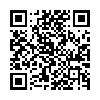
\includegraphics{spayd}
    \caption{SPAYD armazenado num QR Code}
    \label{fig:spayd}
  \end{center}
\end{figure}

\subsection{Pagamentos via NFC} \label{nfc} 

\textit{Near Field Communication} (NFC) é usada maioritariamente para compras feitas em lojas físicas ou serviços de transportes. Um cliente, usando um telemóvel especial equipado com um \textit{smartcard} aproxima o dispositivo de um módulo de leitura. A maioria das transações não requer autenticação, mas algumas fazem-nos através de PIN, antes de completar a transação. O pagamento pode ser deduzido duma conta pré-carregada ou debitada diretamente do saldo do telemóvel ou de uma conta bancária.\cite{SmartCardAlliance2011}
\\Pagamentos móveis através de NFC enfrentam desafios significativos para uma rápida e abrangente adoção, devido à falta de infraestruturas de suporte, ao complexo ecossistema de intervenientes e standards. Apesar disso, alguns produtores de telemóveis e bancos estão entusiasmados com esta tecnologia emergente.\cite{vdc}
\\Os fornecedores de NFC no Japão estão intimamente ligados a redes de trânsito massivo, como por exemplo a Mobile Suica, utilizado na rede férrea JR East. O sistema Osaifu-Keitai, utilizado na Mobile Suica e em muitas outras aplicações, tornou-se o método standard para pagamentos no Japão.
\\Outros fornecedores, principalmente na Europa, usam pagamentos sem contacto através de telemóveis para estacionamento em parques ou na rua em áreas especialmente demarcadas. Os clientes beneficiam porque podem fazer o pagamento no conforto do seu carro com o seu telemóvel, à saída do estacionamento, e os operadores de estacionamento não são obrigados a investir em infraestruturas, novas ou existentes. Os responsáveis pelo estacionamento mantêm a ordem através da matrícula, \textit{transponders} ou códigos de barras. \cite{pargi}
\\Alguns fornecedores usam uma combinação de NFC e código de barras no dispositivo para pagamento, tornando esta técnica mais atrativa nos pontos de venda porque muitos dispositivos móveis no mercado ainda não suportam NFC.\cite{cimbal}

\section{Projetos} \label{projetos}

Segue-se a descrição de alguns projetos existentes, nomeadamente relativos a pagamentos móveis em Portugal. São também apresentados alguns projetos relacionados com bilhética móvel aplicada aos transportes, implementados noutros países.

\subsection{MB Phone}

Lançado em 1996 em Portugal, o MB Phone é um serviço inovador que permite efetuar no telemóvel algumas das operações que, habitualmente, se efetuam no Caixa Automático (normalmente conhecido por multibanco ou ATM). Estas operações têm a particularidade de poderem ser realizadas com ecrãs idênticos aos encontrados nos Caixa Automático, através de uma aplicação Java. Pode ainda utilizar-se o serviço através de serviços de voz ou SMS. 
\\O serviço MB Phone está ativo 24 horas por dia, em Portugal ou em qualquer outro país, com o qual a operadora de telecomunicações tenha acordos de roaming.
\\Ao aliar a mobilidade à funcionalidade, este serviço vai ao encontro do consumidor final mas também dos bancos acionistas que apresentam um serviço que satisfaz as necessidades dos seus clientes. Este serviço está disponível nas operadoras TMN, Vodafone e Optimus e permite as seguintes operações: carregamentos de telemóveis (pré-pagos), pagamentos de serviços, consultas de saldos e movimentos bancários, consultas de NIB, pedidos de livros de cheques e transferência entre contas associadas.\cite{mbphone}
\\A utilização do MB Phone pode ser feita de três maneiras distintas:
\begin{itemize}
\item Aplicação Java – Esta aplicação simula no seu telemóvel os menus de um Caixa Automático;
\item Chamada telefónica – As instruções são dadas durante a chamada;
\item SMS – A mensagem SMS é composta pelos seguintes campos [telecódigo] [cód. da operação] [n.º de seq. da conta] [outros].
\end{itemize}

\begin{figure}[t]
  \begin{center}
    \leavevmode
    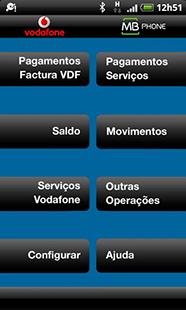
\includegraphics{mbphone}
    \caption{Menu Principal da Aplicação MB Phone para Android}
    \label{fig:mbphone}
  \end{center}
\end{figure}

%%%%%%%%%%%%%%%%%%%%%%%%%%%NEEDS CONFIRMATION
\subsection{WalletPT} 

O WalletPT é uma solução portuguesa inovadora que permite fazer pagamentos em edifícios PT através do telemóvel. Este serviço baseia-se num saldo pré-pago, distinto do saldo de comunicações, que pode carregar-se na página \web através de diversos meios de pagamento, nomeadamente cartão de crédito, PayPal, multibanco ou MB Phone. É este saldo que permite efetuar pagamentos nos vários comerciantes aderentes. Desta forma, é possível controlar eficazmente os gastos, podendo consultar-se todo o histórico de movimentos na página \web ou os mais recentes através do telemóvel. Pode ser efetuada qualquer compra mesmo sem ter dinheiro na carteira.
\\Para se utilizar o serviço é necessário um registo prévio e estão disponíveis quatro formas de pagamento:
\begin{itemize}
\item SMS
\subitem Enviar SMS grátis para o 5665 com "pagar" e será enviado uma mensagem SMS com um código para o telemóvel;
\subitem No ecrã do terminal de pagamento escolher SMS;
\subitem Inserir no terminal de pagamento o código recebido por SMS;
\subitem Selecionar o produto pretendido.
\item USSD
\subitem No ecrã do terminal de pagamento escolher USSD;
\subitem Marcar, no telemóvel, o número indicado no ecrã (*\#566*código*pin de segurança\#);
\subitem Selecionar o produto pretendido.
\item NFC
\subitem Abrir a aplicação WalletPT no telemóvel e inserir o PIN ou aceder à página \web móvel;
\subitem No ecrã do terminal de pagamento escolher Proximidade/NFC;
\subitem Encostar o telemóvel ao terminal de pagamento;
\subitem Introduzir o PIN no telemóvel (apenas necessário se a opção de compras com PIN estiver ativada);
\subitem Selecionar o produto pretendido.
\item QR Code
\subitem Abrir a aplicação WalletPT no telemóvel e inserir o PIN;
\subitem No ecrã do terminal de pagamento escolher Imagem/QR Code;
\subitem Apontar a câmara do telemóvel para o QR Code no terminal de pagamento;
\subitem Confirmar o pagamento no telemóvel;
\subitem Selecionar o produto pretendido.
\end{itemize}
O WalletPT oferece várias vantagens, nomeadamente rapidez, segurança (pagamentos protegidos com PIN de segurança e sem erros de trocos), controlo de gastos, facilidade de utilização e descontos especiais para pagamentos efetuados com o serviço.\cite{walletpt}
%%%%%%%%%%%%%%%%%%%%%%%%%%%

\subsection{Vodafone m.Ticket}

O serviço Vodafone m.ticket powered by ZON Lusomundo (“Vodafone m.Ticket”) é um serviço disponibilizado pela Vodafone Portugal e ZON Lusomundo, que permite aos utilizadores a seleção, aquisição, pagamento e obtenção de bilhetes de cinema para as salas de cinema da ZON Lusomundo, através do telemóvel.
\\O utilizador poderá selecionar o filme, a sala de cinema, a sessão e o número de bilhetes que pretende adquirir através de uma aplicação ou site móvel e efetuar o pagamento do(s) bilhete(s) adquirido(s) através de cartão de crédito ou do sistema de pagamentos MB Phone. Os bilhetes “eletrónicos” são enviados por SMS para o telemóvel do cliente, sob a forma de código alfanumérico (bCode) ou similar e o utilizador valida o(s) bilhete(s) num leitor específico para o efeito (máquina de bCode), localizado na área de acesso às salas de cinema.
\\O Serviço Vodafone m.ticket, na sua vertente de utilização no telemóvel, requer que o utilizador seja detentor de um telefone 3G com capacidade de ligação à Internet.
\\Os preços dos bilhetes adquiridos utilizando o Vodafone m.ticket são ligeiramente inferiores aos praticados nas bilheteiras físicas existentes nos cinemas ZON Lusomundo.\cite{mticket}

\subsection{Transport for London}

Em 2007, um ensaio de NFC para compra de bilhetes de transporte e pequenos pagamentos foi levado a cabo em Londres, o maior ensaio realizado até então. Uma colaboração que envolveu a autoridade de transportes da cidade Transport for London (TfL), a operadora móvel O2, a marca de telemóveis Nokia, o banco Barclays e a empresa de cartões Visa. O objetivo do ensaio era perceber a recetividade dos passageiros a possuírem os cartões, normalmente transportados na carteira, tal como o Oyster (o cartão de transportes no Reino Unido) e cartões de crédito, disponíveis num telemóvel Nokia 6131 equipado com NFC.
\\O ensaio foi um projeto de pesquisa e resposta por parte dos passageiros de grande escala, desenhado para perceber uma série de experiências proporcionadas ao passageiro pelo uso de NFC. Para a TfL era importante perceber como o uso de dispositivos móveis por parte dos passageiros poderia ser uma alternativa potencial aos cartões Oyster.
\\O projeto envolveu 500 clientes da O2, que receberam dispositivos Nokia com funcionalidades NFC. Eram utilizadas três aplicações NFC:
\begin{itemize}
\item O2 – Os participantes podiam usar o seu dispositivo para ganhar entradas no Blueroom, na O2 Arena (o bar exclusivo para clientes da O2 e convidados);
\item Oyster – Os dispositivos do ensaio foram equipados com as funcionalidades Oyster, que permitiam ao participante usar o dispositivo em vez de um cartão Oyster, para carregar títulos de viagem \textit{"pay as you go"} ou títulos semanais ou mensais, e pagar pela viagem no metro, autocarros e comboios existentes na cidade. Cada participante recebeu £50 em crédito para gastar;
\item Pagamentos Barclaycard – Os participantes receberam um saldo de £200 para gastar em pagamentos de baixo valor. Em adição aos pagamentos, os participantes poderiam usar o seu dispositivo para consultar o saldo atual e procurar os lojistas mais próximos que aceitavam pagamentos sem contacto. Esta aplicação foi fornecida através do esquema do cartão Visa, de acordo com os padrões para pagamentos sem contacto.
\end{itemize}
Os principais resultados da pesquisa foram que os participantes mantiveram níveis elevados de interesse e satisfação durante o ensaio e que os principais benefícios para o cliente eram conveniência, facilidade de uso e estatuto.\cite{NFCForum2011} Para além disso referiram que o facto de possuir funcionalidades Oyster seria um fator a ter em conta na compra de um novo telemóvel, e que seria menos propenso a esquecimentos do que um cartão de viagens.
\\De referir, por fim, que existem cerca de vinte mil dispositivos no metro e autocarros de Londres que suportam cartões Oyster e mais de seis milhões de cartões são usados numa base diária.\cite{DeKozan2009} \cite{Mezghani2008}

\subsection{Touch\&Travel}

Touch\&Travel é um projeto piloto de bilhética baseada em NFC, levado a cabo pela Deutsche Bahn, a autoridade alemã dos caminhos de ferro, e pelos parceiros Vodafone, Deutsche Telekom e O2 Germany, com apoio da indústria e companhias locais de transporte. O projeto cobre viagens de longa distância de comboio entre as cidades de Berlim, Colónia, Dusseldorf e Frankfurt, bem como alguns comboios regionais, o metro e elétrico de Berlim, e todos os meios de transporte (incluindo autocarros e \textit{ferry}) da cidade de Potsdam. O projeto teve início em 2008 e em 2011 contava com cerca de três mil participantes a utilizar o serviço com frequência.
\\O objetivo principal deste projeto é testar a viabilidade técnica e a aceitação por parte dos utilizadores de um sistema de entrada/saída baseado em telemóveis com capacidades NFC. Durante o programa piloto, vários dispositivos com NFC das três operadoras foram introduzidos no mercado.
\\As principais vantagens para os participantes do projeto são:
\begin{itemize}
\item Ganham um acesso simples e flexível aos sistemas de transporte de diversas cidades e regiões na Alemanha, independentemente do modo de transporte;
\item Deixam de precisar de comprar bilhetes e ter conhecimento acerca das zonas.
\end{itemize}

Durante o programa piloto, as operadoras distribuíram telemóveis com NFC, equipados com a aplicação Touch\&Travel, residindo a segurança no cartão SIM do telemóvel. O cliente teria de se registar através da Internet e depois disso estava pronto para viajar.
\\Para usar o sistema, o passageiro toca com o seu telemóvel na \textit{tag} NFC na estação de partida. Esta \textit{tag} contém informação relativa ao local. Essa informação é enviada pelo telemóvel, através da rede móvel, para o servidor do sistema Touch\&Travel, que devolve uma confirmação de entrada. Esta confirmação é armazenada no cartão SIM e pode ser acedida por um revisor autorizado com um dispositivo de controlo durante a viagem. No final da viagem, o passageiro necessita de dar saída do sistema, o que é feito através de um novo toque na \textit{tag} NFC da estação de destino. Essa informação é novamente enviada ao servidor e, juntamente com os dados de entrada, é usada para calcular o preço da viagem.
\\Para a Deutsche Bahn, a maior vantagem é a instalação de um sistema de bilhética flexível e escalável, com baixos custos de infraestrutura.\cite{NFCForum2011}

\subsection{Rapid Transit}

Em 2008, a empresa de soluções de pagamento sem contacto ViVOtech desenvolveu um ensaio de pagamento móvel através de NFC em São Francisco (Bay Area Rapid Transit). Em parceria com a Sprint, a First Data, a cadeia de restaurantes \textit{fast-food} Jack in the Box, o projeto permitiu a centenas de passageiros viajar na rede apenas tocando com o seu dispositivo móvel com NFC nos portões de acesso às estações.
\\Este ensaio foi o primeiro nos Estados Unidos da América a combinar viagens baseadas em bilhetes móveis com pagamentos móveis em lojas associadas, permitindo aos utilizadores pagarem refeições nos restaurantes Jack in the Box. Para além disso, o ensaio incluía promoções em posters inteligentes que ajudavam os utilizadores a dirigirem-se à loja referenciada.
\\O ensaio foi um grande sucesso, com um número elevado de utilização por parte dos utilizadores, tanto no sistema de transportes como na cadeia de restaurantes.\cite{NFCForum2011} \cite{Casey2000}

\subsection{Mobipay}

Mobipay é um sistema espanhol que ativa os meios de pagamento existentes (crédito normal ou virtual, débito ou cartões pré-pagos) e que permite efetuar uma série de operações no telemóvel. Pode, por exemplo, ser usado para realizar compras na Internet, pagar um táxi, carregar um cartão pré-pago, viajar nos transportes públicos, transferir dinheiro para outra pessoa, etc.
\\Os utilizadores podem optar por associar o seu cartão de crédito ou débito Visa ou MasterCard à sua conta Mobipay e realizar os pagamentos diretamente do cartão ou então, em compras pequenas (menos de \euro 6), podem deduzir diretamente do saldo do cartão SIM.
\\Mobipay surge duma parceria conjunta entre todas as operadoras móveis espanholas e 80\% das instituições financeiras. O objetivo é lançar os serviços de comércio móvel em Espanha e transformar o dispositivo móvel num meio de pagamento seguro, flexível e intuitivo. \cite{atos}

\subsection{ÖBB SMS-Ticket}

O operador de caminhos de ferro austríaco, ÖBB, possui um serviço de bilhetes via SMS, que podem facilmente ser obtidos pelos seus passageiros através do telemóvel. O custo da operação é debitado diretamente do saldo do cartão SIM, caso seja um utilizador da operadora móvel A1, ou das contas bancárias associadas, no caso das outras operadoras móveis.
\\O utilizador envia uma SMS com a palavra ZUG e a seguinte lista de parâmetros (separados por espaço):
\begin{itemize}
\item Estação de partida;
\item Estação de destino;
\item Primeiro e último nome;
\item Número de adultos (opcional);
\item Número de crianças (opcional);
\item Cartão VORTEILS (cartão que oferece vantagens, nomeadamente desconto no preço) (opcional);
\item Classe (1ª ao 2ª) (opcional);
\item Data da Viagem (opcional).
\end{itemize}
Recebe seguidamente uma SMS contendo o resumo da viagem e a indicação do preço. Para confirmar a compra basta responder à SMS.
\\Por fim, apenas alguns segundos depois, o utilizador recebe o bilhete via SMS e deverá mantê-la até ao final da viagem, como prova de validade. \cite{obb}

\subsection{Mobill} 

A Mobill Scandinavia AB é uma empresa de software relacionada com comércio móvel, com base em Malmö, na Suécia. A Mobill apresenta cinco soluções diferentes para áreas distintas do comércio móvel; pagamentos,  estacionamento, bilhetes, cupões e eventos.\cite{mobill}
\begin{itemize}
\item \emph{M-Payment} é uma aplicação altamente configurável que suporta um vasto leque de cenários onde bens e serviços são comprados utilizando um telemóvel. M-Payment inclui APIs para integração com máquinas de venda, páginas \web e terminais de pontos de venda;
\item \emph{M-Parking} é a solução da Mobill para pagamentos fáceis de estacionamento através do telemóvel, com lembretes automáticos quando o tempo se aproxima do fim e a possibilidade de remotamente prolongar o período inicialmente selecionado. M-Parking é usado por mais de cinquenta empresas de parques automóveis na Suécia.
\item \emph{M-Ticket} permite aos clientes comprar bilhetes de transportes públicos (autocarro, elétrico, metro, comboio) através do telemóvel e recebê-los diretamente no dispositivo. Os bilhetes podem ser automaticamente digitalizados e validados usando a tecnologia Mcode da Mobill.
\item \emph{M-Gateway} permite aos vendedores enviar mensagens e cupões eletrónicos usando listas de clientes ou a API em tempo real. Os cupões podem integrar a tecnologia Mcode para automaticamente serem validados pelos dispositivos de leitura e assim obter resultados em tempo real.
\item \emph{M-Event} fornece bilhetes eletrónicos seguros que podem ser validados na entrada do evento. A tecnologia Mcode permite que os bilhetes sejam validados diretamente do ecrã do telemóvel do utilizador.
\end{itemize}
A tecnologia Mcode referida baseia-se num bloco compacto de caracteres para codificar o número identificativo do bilhete. É otimizado para caber no ecrã do telemóvel e facilitar uma leitura fiável. O sistema de produção usa um esquema de codificação que fornece uma base de códigos suficiente para uma utilização em larga escala, sem repetições. Um exemplo pode ser visto na Figura~\ref{fig:mcode}.

\begin{figure}[t]
  \begin{center}
    \leavevmode
    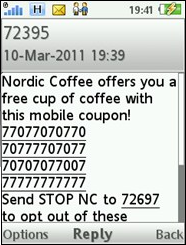
\includegraphics{mcode}
    \caption{Mcode contendo um cupão}
    \label{fig:mcode}
  \end{center}
\end{figure}

\section{Resumo}

O uso de telemóveis em sistemas de transporte público está a aumentar. Os operadores começaram por implementar funcionalidades básicas, como por exemplo o envio de mensagens SMS para consulta de informação, e agora começam a evoluir para processos mais complexos como a compra de títulos de viagem ou até o cálculo automático do preço baseado no percurso efetuado.
\\Com a evolução dos telemóveis e a adição de tecnologias como NFC, adicionar as referidas funcionalidades torna-se mais fácil e viável. Os bilhetes podem ser comprados, descarregados e acedidos através do telemóvel e validados com um simples toque num leitor com tecnologia NFC, emitindo automaticamente uma confirmação. São já várias as redes de transporte a efetuar testes com sistemas de bilhética móvel, ou seja, deixando de parte os cartões físicos e passando todo o processo a ser realizado no dispositivo móvel.
\\Para além disso podem usar-se outras funcionalidades do telemóvel, como por exemplo o ecrã para visualização de bilhetes virtuais, o GPS para determinar a posição atual do passageiro, navegador \textit{web}, câmara, som, etc., para fornecer serviços adicionais aos passageiros, melhorando a experiência de viagem dos passageiros. Partindo desta premissa, o modelo tradicional de serviços de transporte é melhorado com acesso a informação de trânsito e horários em tempo real, possibilidade de consultar instantaneamente o saldo de viagens, planear de forma interativa uma viagem, partilhar opiniões e trajetos com outros passageiros, entre outras possíveis funcionalidades.\cite{Nunes2011}
\\Os telemóveis possuem várias características que os tornam únicos e adequados para serem usados para pagamentos e proporcionarem serviços adicionais: estão ligados à rede constantemente, possuem interfaces de som e texto familiares e fáceis de usar, permitem um acesso a informação em qualquer altura em qualquer lugar, as aplicações são fáceis de descarregar e instalar.
\\Comparando os telemóveis com bilhetes magnéticos no contexto dos transportes públicos, os telemóveis permitem um acesso remoto e ubíquo a serviços de pagamento, eliminando assim a necessidade de esperar numa fila e a necessidade de pagar em dinheiro. Isto é especialmente importante em certas situações em que o passageiro não dispõe de muito tempo disponível antes de iniciar a sua viagem ou não possui dinheiro consigo para efetuar o pagamento.\cite{Mallat2007}
\\Um outro fator importante é o facto de ser menos provável perder o telemóvel do que um bilhete e vários estudos mostram que é menos provável as pessoas saírem de casa sem do telemóvel do que sem a carteira. Adicionalmente, bilhetes em papel acabam por se estragar com o uso intensivo e necessitam de ser substituídos com frequência, o que faz dos bilhetes móveis mais robustos e convenientes, para além de serem uma melhor solução a nível ambiental.
\\Os telemóveis possuem também vantagens em comparação com os cartões sem contacto. Ao contrário destes, o telemóvel pode suportar mais do que um título diferente de mais do que um operador de transportes, enquanto os cartões sem contacto, por norma, apenas permitem um tipo de bilhete, obrigado o passageiro a carregar consigo uma série de cartões diferentes. Isto faz com que, numa carteira com vários cartões, seja necessário retirar o cartão desejado antes de o apresentar à máquina de leitura. Caso contrário, provavelmente não será possível ler o cartão ou será validado um cartão que não o desejado. Em adição a isso, os passageiros podem gerir os seus cartões e bilhetes em qualquer altura em qualquer lugar. Por exemplo, as assinaturas mensais podem ser renovadas sem necessidade de esperar em filas.\cite{NFCForum2011}
\\Por fim, com a gestão feita diretamente no telemóvel do passageiro, é possível aos operadores de transportes públicos interagir com os seus passageiros fazendo sugestões baseadas no perfil de utilização ou oferecer descontos especiais ou pontos de lealdade.\cite{Ferreira2012}
\chapter{Sistema Andante}\label{chap:andante}

\section*{}

Neste capítulo é detalhado o sistema Andante, utilizado nos transportes públicos de passageiros da Área Metropolitana do Porto, permitindo contextualizar os conceitos e modalidades utilizados na aplicação.
\\O Andante é um título que permite viajar em diversos transportes públicos, de diferentes operadores, sendo o preço calculado baseado no trajeto a efetuar e não no modo de transporte utilizado ou o número de embarques realizados.
\\Os operadores aderentes ao sistema Andante são: Metro do Porto, STCP - Sociedade de Transportes Coletivos do Porto, CP - Comboios de Portugal, Resende, Espírito Santo, Maia Transportes, Valpi, Gondomarense, MGC Transportes, Nogueira da Costa e Auto-Viação Pacense. 

\section{Modalidades}

Os títulos Andante dividem-se em dois grandes grupos: Ocasionais e Assinaturas.

\subsection{Ocasionais}

Os títulos ocasionais estão disponíveis em duas alternativas: Título de Viagem e Andante 24. Tanto uma como outra utilizam o cartão azul, em papel, que não é personalizado e como tal permite a utilização por mais do que uma pessoa, desde que não seja em simultâneo.

\subsubsection{Título de Viagem}

Permite viajar durante um determinado período de tempo consoante o número de zonas compradas (Z2 – 2 anéis de zonas; Z3 – 3 anéis de zonas; e assim sucessivamente).
\\O mínimo de tempo que um título de viagem permite andar é de 1 hora. Este tempo de viagem aumenta à medida que cresce o número de zonas carregadas.

\subsubsection{Andante 24}

O funcionamento do Andante 24 é semelhante ao título de viagem, com a diferença de independentemente do número de zonas carregadas, permitir viajar durante as vinte e quatro horas seguintes à primeira validação.

\subsubsection{Andante Tour}

Título de transporte vocacionado para o segmento de turistas, confere acesso a toda a rede Andante permitindo um número ilimitado de viagens durante 24 horas (Andante Tour 1) ou 72 horas (Andante Tour 3) consecutivas após a primeira validação.
\\O cartão Andante Tour não é recarregável.


\subsection{Assinaturas}

As assinaturas permitem ao utilizador viajar dentro das zonas previamente selecionadas durante o período equivalente ao mês de calendário. Ao contrário dos títulos ocasionais, é necessário especificar quais as zonas pretendidas e a assinatura é apenas válida nessas zonas. O cartão da assinatura é o dourado, em plástico, e para além de fotografia inclui também o nome do utilizador, tornando-o de uso pessoal e intransmissível.
\\As assinaturas têm tarifas especiais para jovens, estudantes, reformados, pensionistas, seniores e beneficiários de ação social.

\section{Zonamento}

A rede de transportes públicos da Área Metropolitana do Porto está divida por zonas. Cada zona é constituída por uma letra e um número. As zonas estão agrupadas em três grandes grupos (Norte, Centro e Sul) e a inicial desse grupo serve para identificar a zona (N, C, S). Dentro de cada grupo as zonas são depois numeradas sequencialmente. Pode ver-se na Figura~\ref{fig:zonas} o zonamento Andante.
\\Este mapa é especialmente importante para perceber o número de zonas a carregar num título ocasional. Por exemplo, com um título Z2, entrando na zona C1 (centro do Porto), é possível viajar dentro dessa zona e em todas as que lhe sejam adjacentes (C2, C6 e S8). Por outro lado, usando um título Z3, pode viajar-se também até ao segundo anel de adjacência (C3, C5, C7, C8, C9, S1, S2, S7, S9). Ver Figura~\ref{fig:zonas_c1}.

\begin{figure}[t]
  \begin{center}
    \leavevmode
    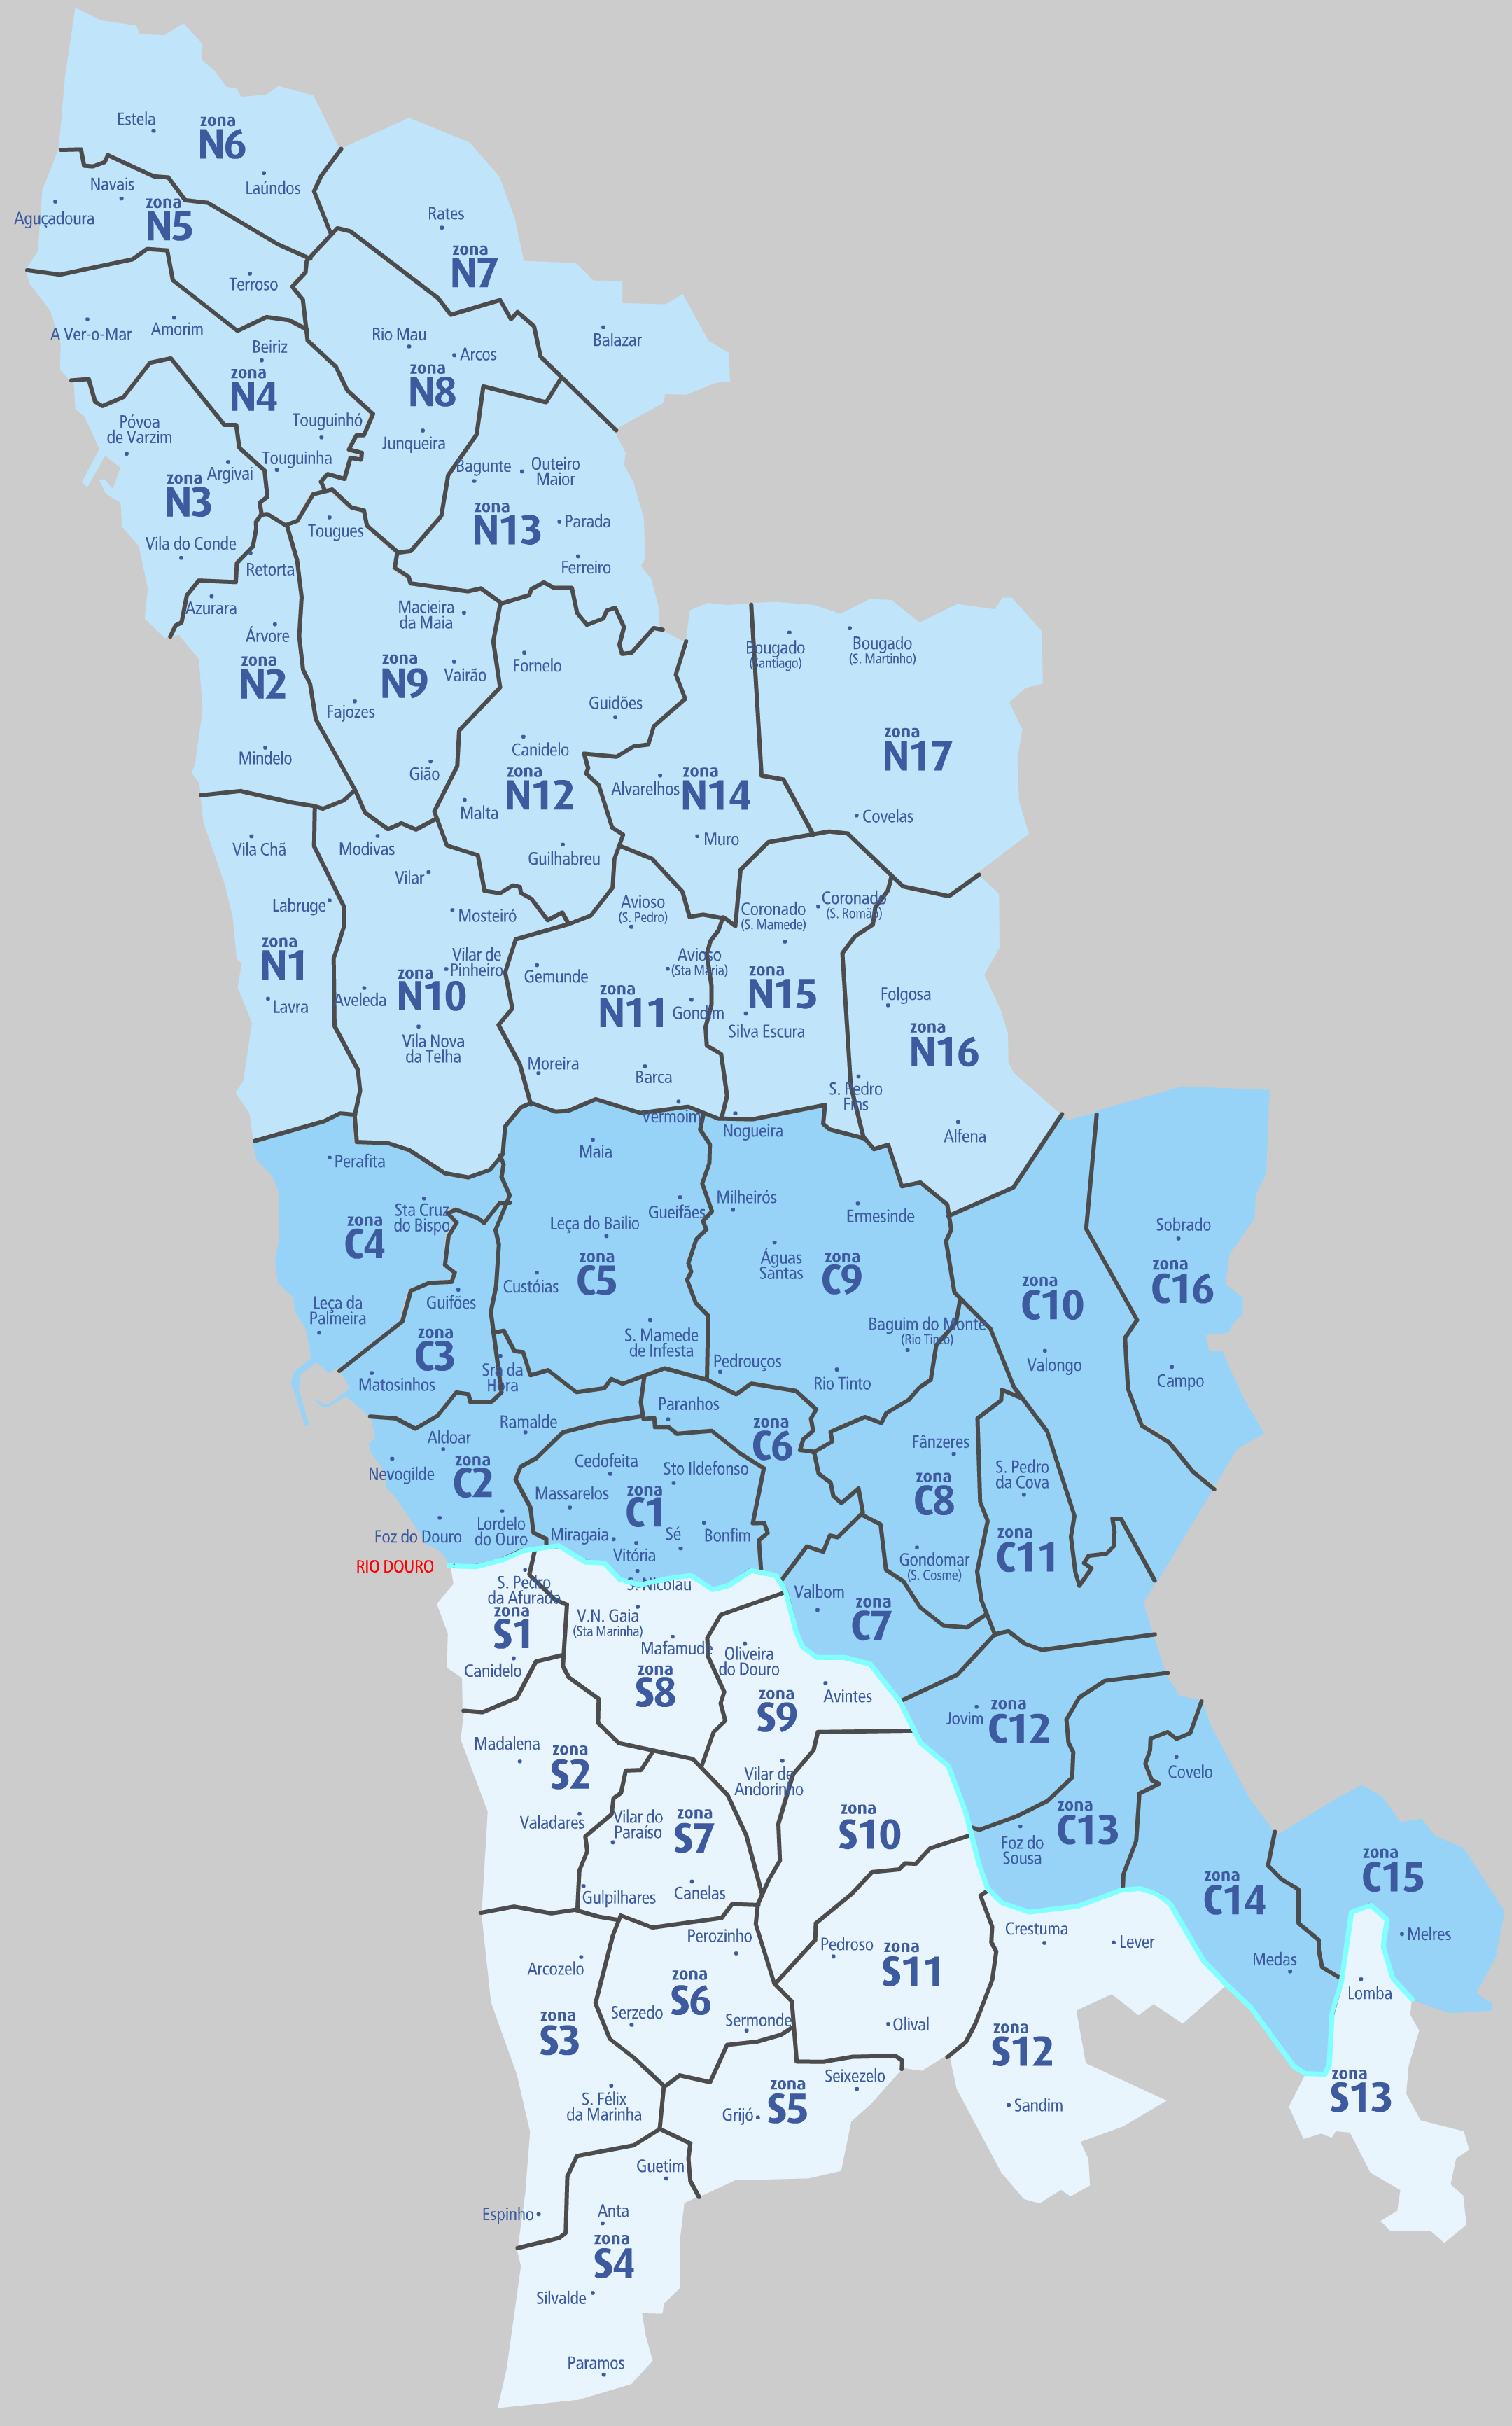
\includegraphics[scale=0.375]{zonas}
    \caption{Zonamento Andante}
    \label{fig:zonas}
  \end{center}
\end{figure}

\begin{figure}[t]
  \begin{center}
    \leavevmode
    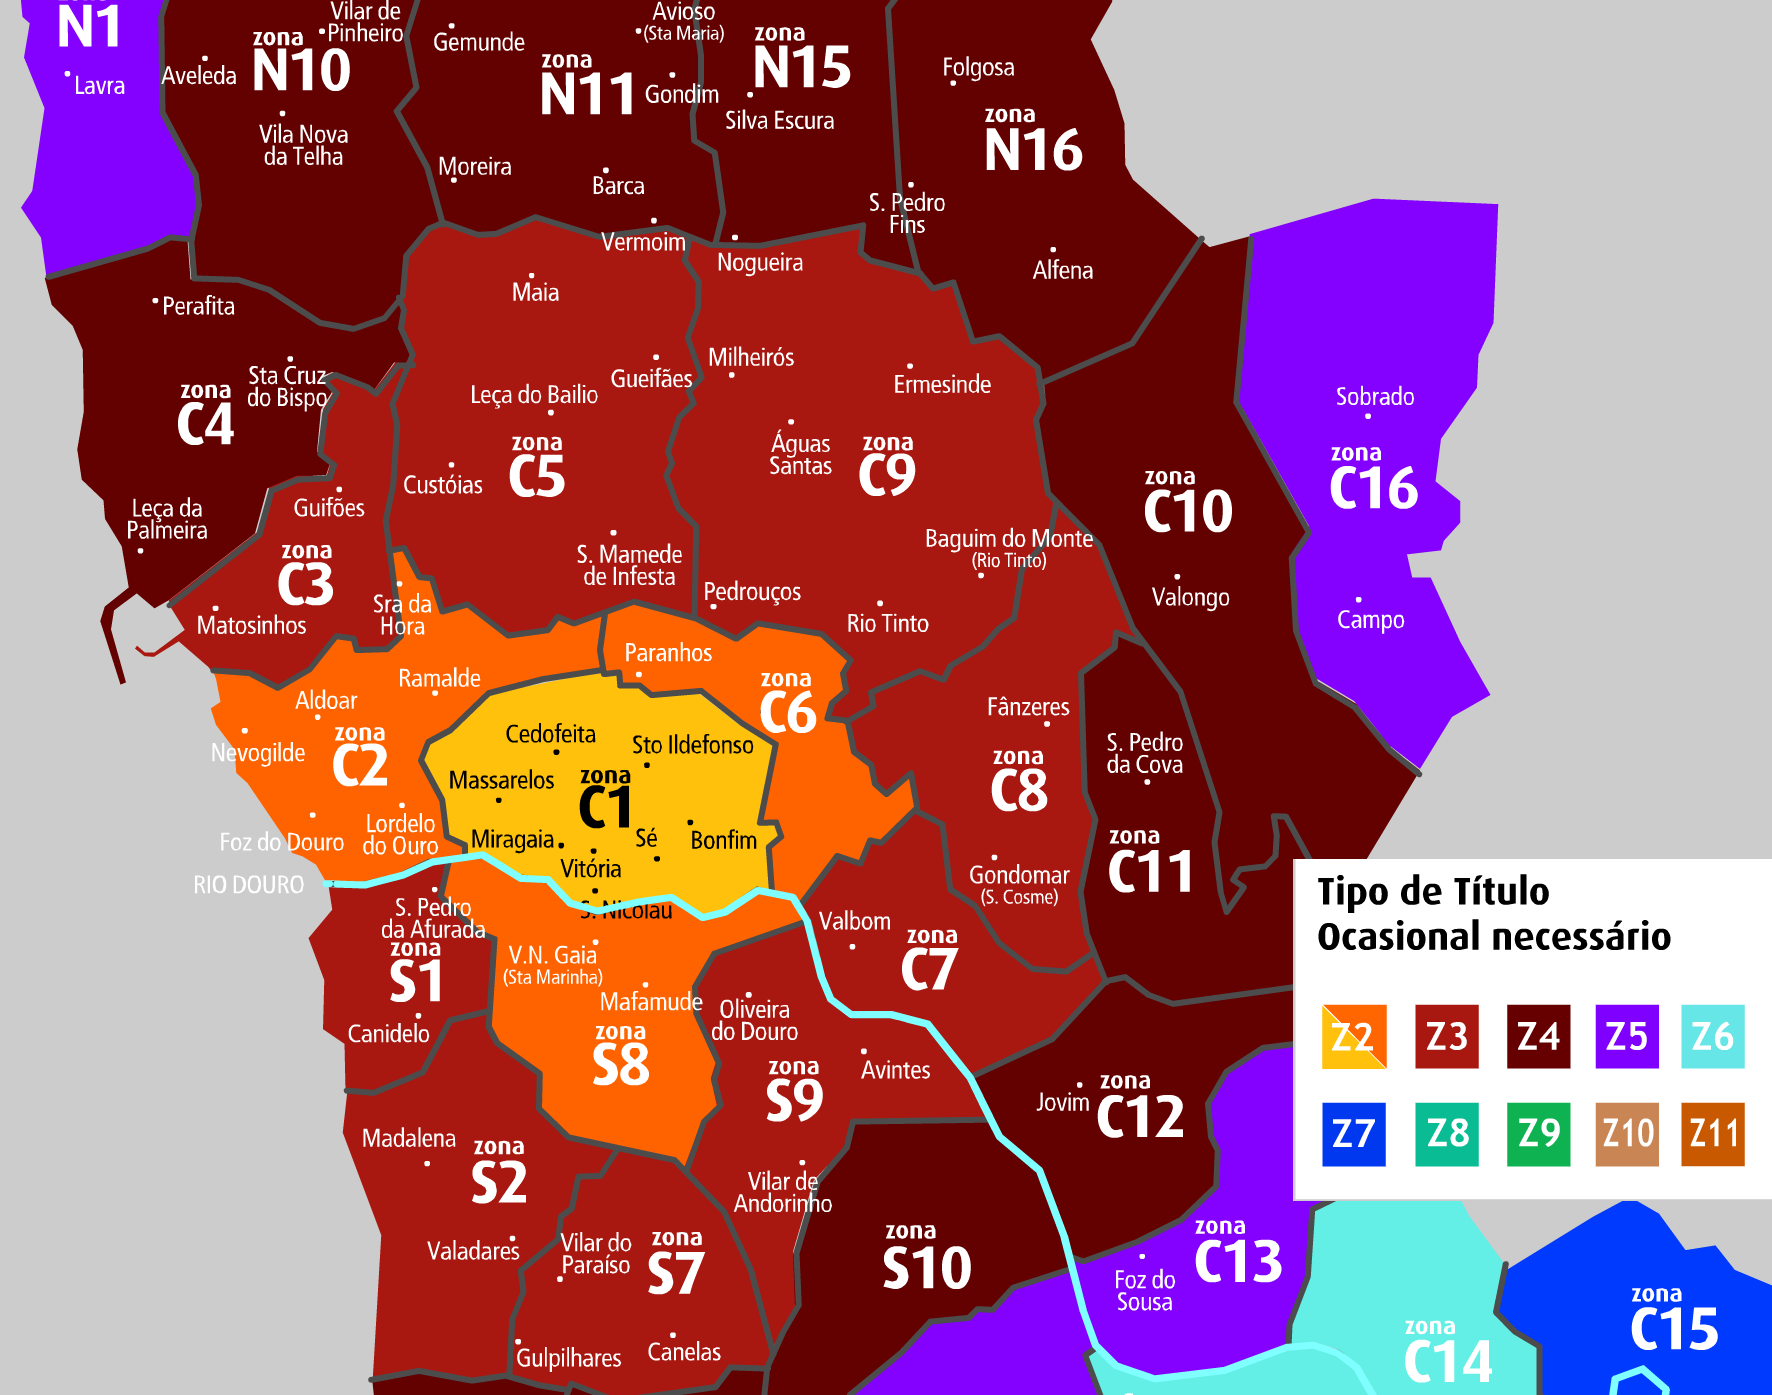
\includegraphics[scale=0.5]{zonas_c1}
    \caption{Cálculo de número de zonas Andante \cite{calczonas}}
    \label{fig:zonas_c1}
  \end{center}
\end{figure}

\section{Resumo ou Conclusões}

O sistema Andante traz aos transportes públicos da Área Metropolitana do Porto a comodidade e rapidez de utilizar apenas um só método de bilhética, permitindo aos operadores ter um sistema standard e familiar para o utilizador.
\\No entanto, muitas vezes os utilizadores ocasionais (turistas, por exemplo) têm alguma dificuldade em perceber o funcionamento do sistema Andante devido à sua complexidade, nomeadamente ao cálculo de zonas necessárias para efetuar determinada viagem. Sendo que uma viagem poderá necessitar de número de zonas diferentes consoante o sentido em que é feito, devido ao facto de os percursos de ida e volta nem sempre coincidirem.
\chapter{Implementação}\label{chap:implement}

\section*{}

Neste capítulo é especificado de forma detalhada o desenvolvimento e implementação do protótipo desenvolvido, bem como as suas principais características. Pretende-se apresentar as várias fase de desenvolvimento e, em cada uma delas, o trabalho realizado e as conclusões retiradas, tendo em vista uma melhoria constante do produto final.

\section{Especificação de Requisitos}

Para desenvolver uma aplicação que se adequasse às necessidades reais dos utilizadores e das entidades envolvidas, foi necessário analisar o sistema de bilhética atual e perceber quais as ações fundamentais para uma implementação eficaz. Para além disso, foi também necessário avaliar quais as principais funcionalidades que trariam valor ao serem implementadas e que tirariam o máximo proveito das capacidades dos dispositivos móveis. Em anexo encontra-se a especificação detalhada dos requisitos funcionais. Ver Anexo~\ref{rer}.

\subsection{Requisitos Funcionais}

Começando pelos requisitos relacionados com a utilização de autenticação de utilizadores, salvaguardando assim os dados pessoais e permitindo a segurança das operações efetuadas, definiram-se como requisitos funcionais os seguintes:
\begin{itemize}
\item O sistema deve permitir o registo de um novo utilizador;
\item O sistema deve permitir a autenticação de um utilizador já registado;
\item O sistema deve permitir a um utilizador autenticado alterar os seus dados pessoais;
\item O sistema deve permitir a um utilizador autenticado terminar a sessão ativa.
\end{itemize}

Os requisitos funcionais relacionados com o funcionamento de um sistema de bilhética são os seguintes:
\begin{itemize}
\item O sistema deve permitir a compra de títulos por utilizadores autenticados;
\item O sistema deve utilizar os fornecedores de localização do dispositivo móvel para identificar a paragem onde o utilizador autenticado se encontra;
\item O sistema deve permitir ao utilizador autenticado a escolha manual da paragem de entrada;
\item O sistema deve listar as linhas e respetivos sentidos que passam na paragem selecionada pelo utilizador autenticado;
\item O sistema deve permitir ao utilizador autenticado escolher o título a validar, apresentando todos os títulos disponíveis que se adequem à paragem e linha selecionadas;
\item O sistema deve permitir ao utilizador autenticado efetuar a validação do título escolhido, apresentando a paragem limite até à qual pode viajar;
\item O sistema deve permitir a mudança de linha (transbordo), quando existir um título válido;
\item O sistema deve permitir a confirmação da validade do título em utilização, por parte do revisor.
\end{itemize}

Por fim, os requisitos funcionais relacionados com a visualização de informação por parte do utilizador:
\begin{itemize}
\item O sistema deve permitir a consulta do estado atual do título validado;
\item O sistema deve permitir o acesso ao histórico de operações efetuadas pelo utilizador autenticado;
\item O sistema deve permitir o acesso ao histórico de validações realizadas pelo utilizador autenticado;
\item O sistema deve permitir a consulta do saldo de títulos disponíveis;
\item O sistema deve permitir a consulta de saldo da carteira virtual.
\end{itemize}

\subsection{Requisitos Não Funcionais}

Para além dos requisitos acima especificados, foram também delineadas algumas características que a aplicação deve conter:
\begin{itemize}
\item Comunicação - É necessário uma ligação à rede com um acesso estável e com uma largura de banda mínima que permita a plena utilização de todas as funcionalidades disponíveis;
\item Eficiência - Uma normal utilização do sistema requer inúmeros acessos simultâneos à aplicação e, consequentemente, à sua base de dados. Logo, é fulcral que a aplicação esteja estruturada para que a informação seja acedida e apresentada em tempos de resposta mínimos, de modo a que o utilizador veja satisfeitos os seus propósitos de manipulação de informação;
\item Fiabilidade - O sistema deverá garantir a integridade dos dados submetidos;
\item Manutenção - O sistema deverá permitir uma fácil manutenção e adição de novas funcionalidades;
\item Segurança - O sistema deve estar devidamente protegido para que não haja a possibilidade de acessos indevidos a dados confidenciais dos utilizadores.
\item Usabilidade - Pretende-se que a interface da aplicação seja intuitiva e de fácil utilização, para que o utilizador não perca muito tempo no processo de aprendizagem do manuseamento da mesma. É importante também que o número de cliques para execução das ações seja o menor possível, reduzindo assim o tempo de execução. O sistema deverá, também, oferecer mensagens de erro claras e ajuda contextual;
\item Compatibilidade - O sistema deverá funcionar perfeitamente em dispositivos Android com verão 2.2 (API 8) ou superior. Para além disso, o sistema deverá ter uma integração coerente com a aplicação MOVE-ME.

\end{itemize}

\section{Mais uma Secção}


%\begin{lstlisting}[float,language=Java, label=src:mapreduce, caption=Example map and reduce functions for word counting]
%map(String key, String value): 
%// key: document name 
%// value: document contents 
%for each word w in value:
%EmitIntermediate(w, "1");
%
%reduce(String key, Iterator values):
%// key: a word 
%// values: a list of counts 
%int result = 0;
%for each v in values: 
%result += ParseInt(v);
%
%Emit(AsString(result))
%\end{lstlisting}


\section{Resumo ou Conclusões}
%\chapter{Implementação}\label{chap:chap4}

\section*{}

Este capítulo pode ser dedicado à apresentação de detalhes de nível
mais baixo relacionados com o enquadramento e implementação das
soluções preconizadas no capítulo anterior.
Note-se no entanto que detalhes desnecessários à compreensão do
trabalho devem ser remetidos para anexos.

Dependendo do volume, a avaliação do trabalho pode ser incluída neste
capítulo ou pode constituir um capítulo separado.

\section{Secção Exemplo}

%\todofigure{Inserir uma figura sobre o Map/Reduce}

Lorem ipsum dolor sit amet, consectetuer adipiscing elit. Integer
hendrerit commodo ante. Pellentesque nibh libero, aliquam at, faucibus
id, commodo a, velit. 
%\todoline{Escrever sobre o map/reduce}
Duis eleifend sem eget leo. Morbi in est. Suspendisse magna sem,
varius nec, hendrerit non, tincidunt quis, quam. Aenean congue. 
%\todolines{A short entry in the list of todos}{A very long todonote
%  that certainly will fill more than a single line in the list of
%  todos. Just to make sure let's add some more text.} 
Vivamus vel est sit amet sem iaculis posuere. Cras mollis, enim vel
gravida aliquam, libero nunc ullamcorper dui, ullamcorper sodales
lectus nulla sed urna. Morbi aliquet porta risus. 
Proin vestibulum ligula a purus. Maecenas a nulla. 
Maecenas mattis est vitae neque auctor tempus. Etiam nulla dui,
mattis vitae, porttitor sed, aliquet ut, enim. Cras nisl magna,
aliquet et, laoreet at, gravida ac, neque. Sed id est. Nulla dapibus
dolor quis ipsum rhoncus cursus. 

\section{Mais uma Secção}

Lorem ipsum dolor sit amet, consectetuer adipiscing elit. Quisque
purus sapien, interdum ut, vestibulum a, accumsan ullamcorper,
erat. Mauris a magna ut leo porta imperdiet. Donec dui odio, porta in,
pretium non, semper quis, orci. Quisque erat diam, pharetra vel,
laoreet ac, hendrerit vel, enim. Donec tristique luctus risus. Fusce
dolor est, eleifend id, elementum sit amet, varius vitae, neque. Morbi
at augue. Ut sem ligula, auctor vitae, facilisis id, pharetra non,
lectus. Nulla lacus augue, aliquam eget, sollicitudin sed, hendrerit
eu, leo. Suspendisse ac tortor. Mauris at odio. Etiam vehicula. Nam
lacinia purus at nibh. Aliquam fringilla lorem ac justo. Ut nec
enim. 
%\todoref{Citar Map/reduce}

Quisque ullamcorper. Aliquam vel magna. Sed pulvinar dictum
ligula. Sed ultrices dolor ut turpis. Vivamus sagittis orci malesuada
arcu venenatis auctor. Proin vehicula pharetra urna. Aliquam egestas
nunc quis nisl. Donec ullamcorper. Nulla purus. Ut suscipit lacus
vitae dui. Mauris semper. Ut eget sem. Integer orci. Nam vitae dui
eget nisi placerat convallis. 

\begin{lstlisting}[float,language=Java, label=src:mapreduce, caption=Example map and reduce functions for word counting]
map(String key, String value): 
// key: document name 
// value: document contents 
for each word w in value:
EmitIntermediate(w, "1");

reduce(String key, Iterator values):
// key: a word 
// values: a list of counts 
int result = 0;
for each v in values: 
result += ParseInt(v);

Emit(AsString(result))
\end{lstlisting}

Sed id lorem. Proin gravida bibendum lacus. Sed molestie, urna quis
euismod laoreet, diam dolor dictum diam, vitae consectetuer leo ipsum
id ante. Integer eu lectus non mauris pharetra viverra. In feugiat
libero ut massa. Morbi cursus, lorem sollicitudin blandit semper,
felis magna pellentesque lacus, ut rhoncus leo neque at tellus. Sed
mattis, diam eget eleifend tincidunt, ligula eros tincidunt diam,
vitae auctor turpis est vel nunc. In eu magna. Donec dolor metus,
egestas sit amet, ultrices in, faucibus sed, lectus. Etiam est enim,
vehicula pharetra, porta non, viverra vel, nunc. Ut non sem. Etiam nec
neque. 

\section{Resumo ou Conclusões}

Proin vehicula pharetra urna. Aliquam egestas
nunc quis nisl. Donec ullamcorper. Nulla purus. Ut suscipit lacus
vitae dui. Mauris semper. Ut eget sem. Integer orci. Nam vitae dui
eget nisi placerat convallis. 
 

%%----------------------------------------
%% Final materials
%%----------------------------------------

%% Bibliography
%% Comment the next command if BibTeX file not used, 
%% Assumes that bibliography is in ``myrefs.bib''
\PrintBib{refs}

%% Comment next 2 commands if numbered appendices are not used
\appendix
\chapter{Planeamento (Parte 1)} \label{gantt1}

O período apresentado refere-se aos meses de novembro de 2012 a fevereiro de 2013, coincidindo com a Unidade Curricular EIC0087 - Preparação da Dissertação.

\begin{figure}[t]
  \begin{center}
    \leavevmode
    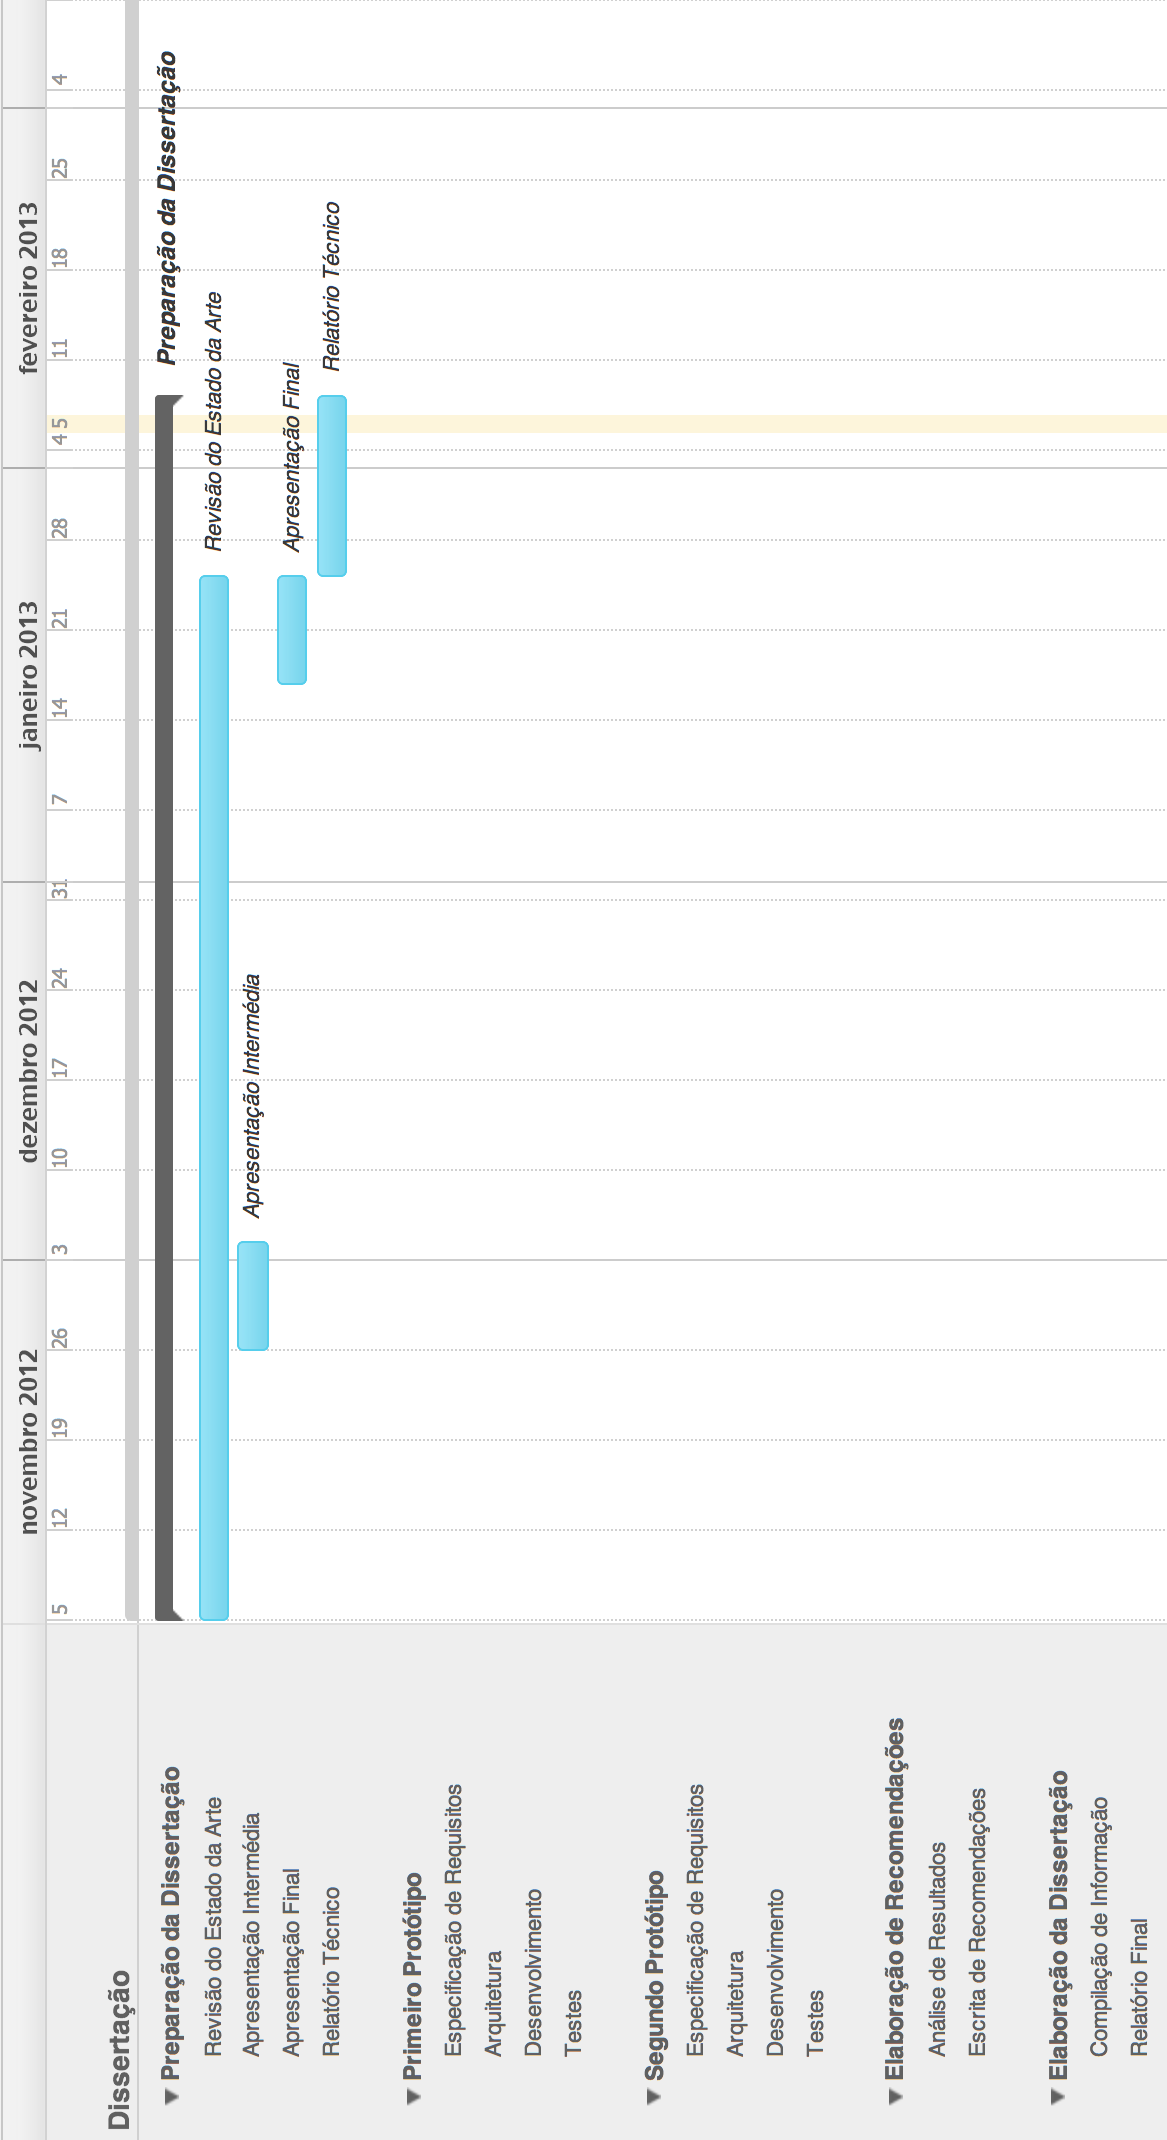
\includegraphics[height=23cm]{gantt_part1}
    \caption{Planeamento da primeira fase da dissertação}
    \label{fig:gantt1}
  \end{center}
\end{figure}

\chapter{Planeamento (Parte 1)} \label{gantt1}

O período apresentado refere-se aos meses de novembro de 2012 a fevereiro de 2013, coincidindo com a Unidade Curricular EIC0087 - Preparação da Dissertação.

\begin{figure}[t]
  \begin{center}
    \leavevmode
    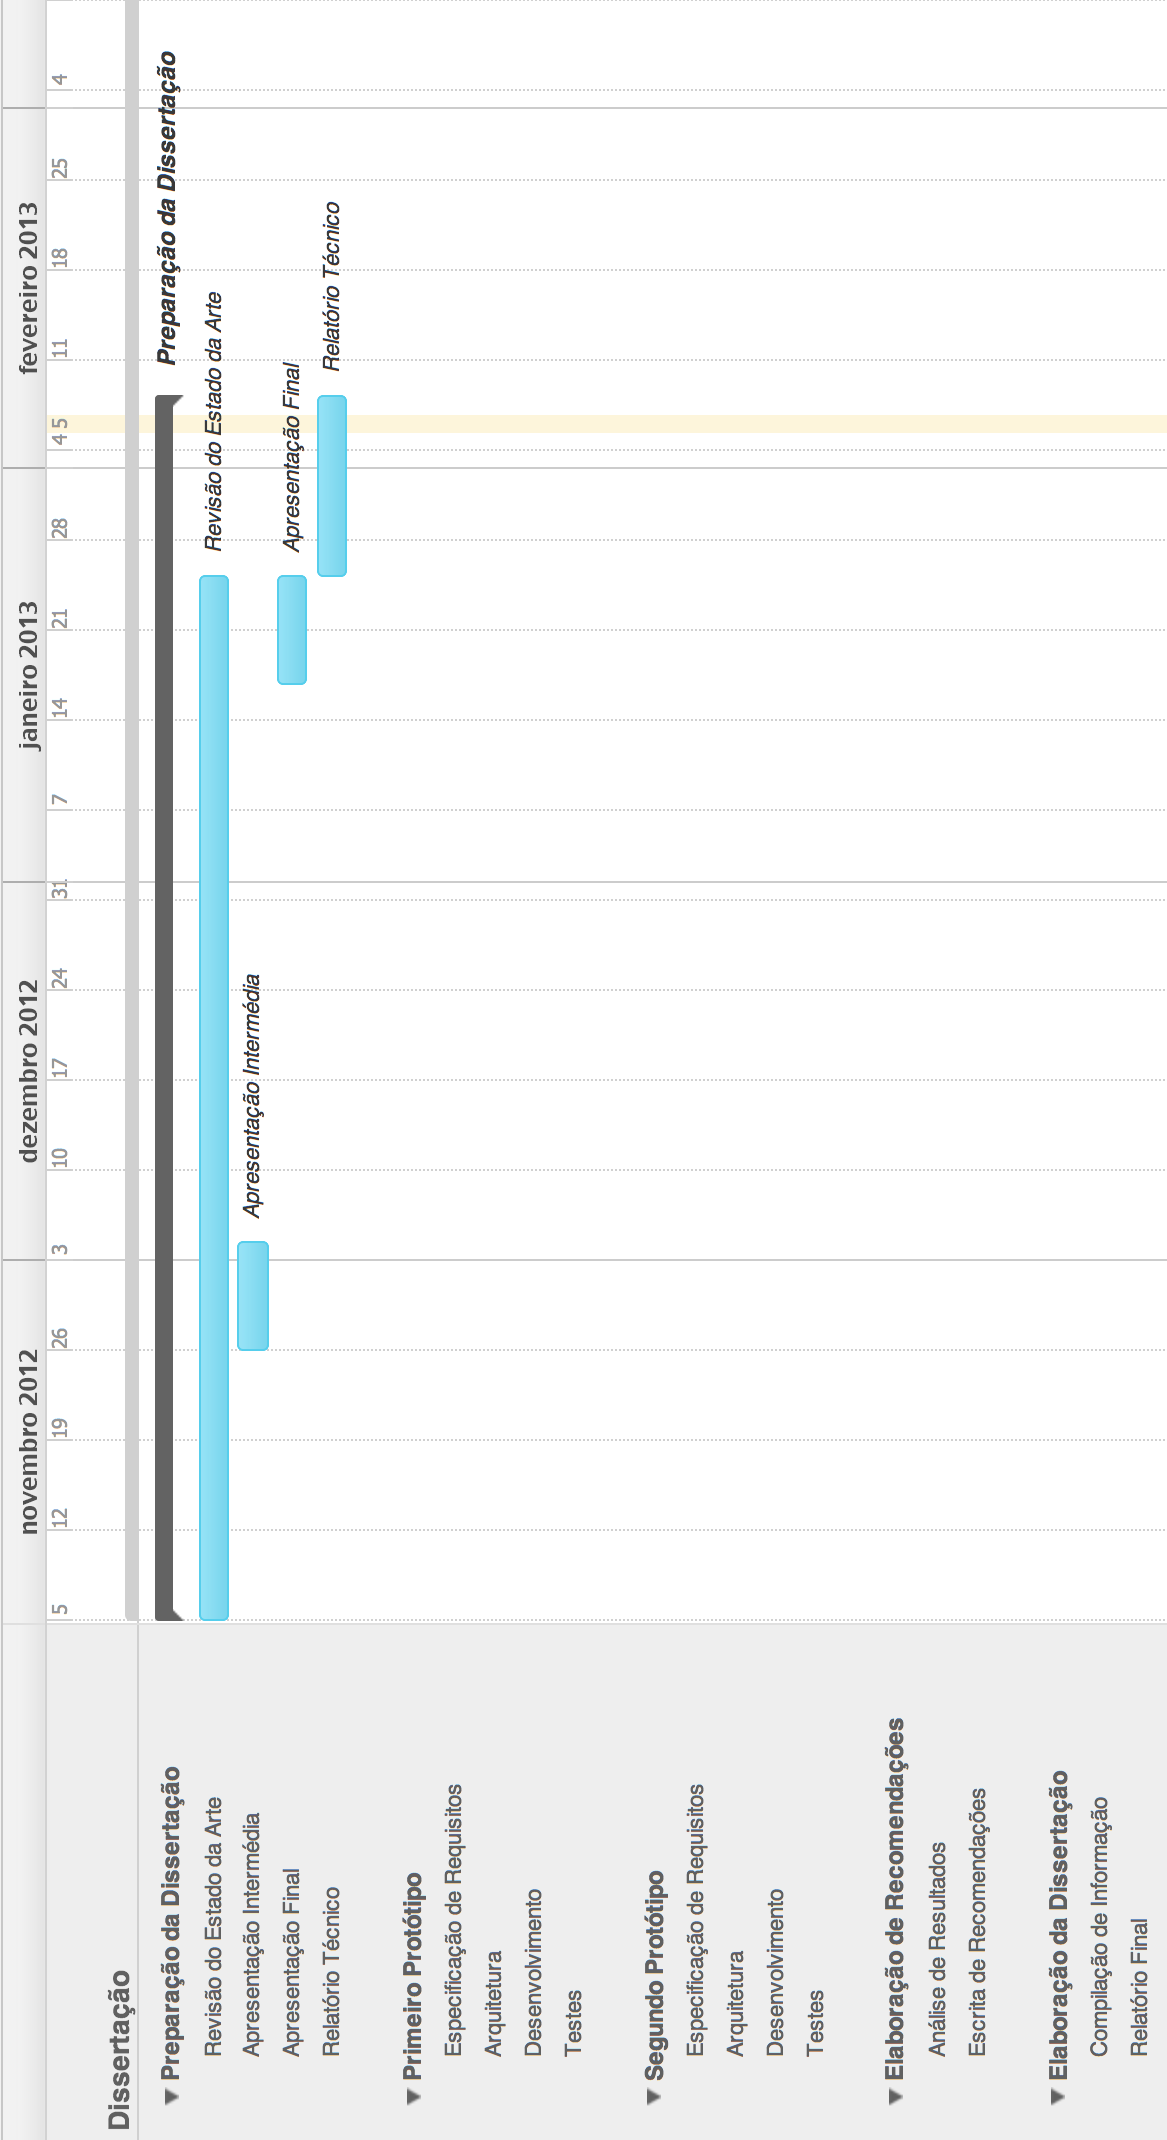
\includegraphics[height=23cm]{gantt_part1}
    \caption{Planeamento da primeira fase da dissertação}
    \label{fig:gantt1}
  \end{center}
\end{figure}


%% Index
%% Uncomment next command if index is required, 
%% don't forget to run ``makeindex mieic'' command
%\PrintIndex

\end{document}
